\chapter{Conceptos fundamentales de TikiWiki}
\label{chapter:conceptos-fundamentales-tiki}

\begin{center}
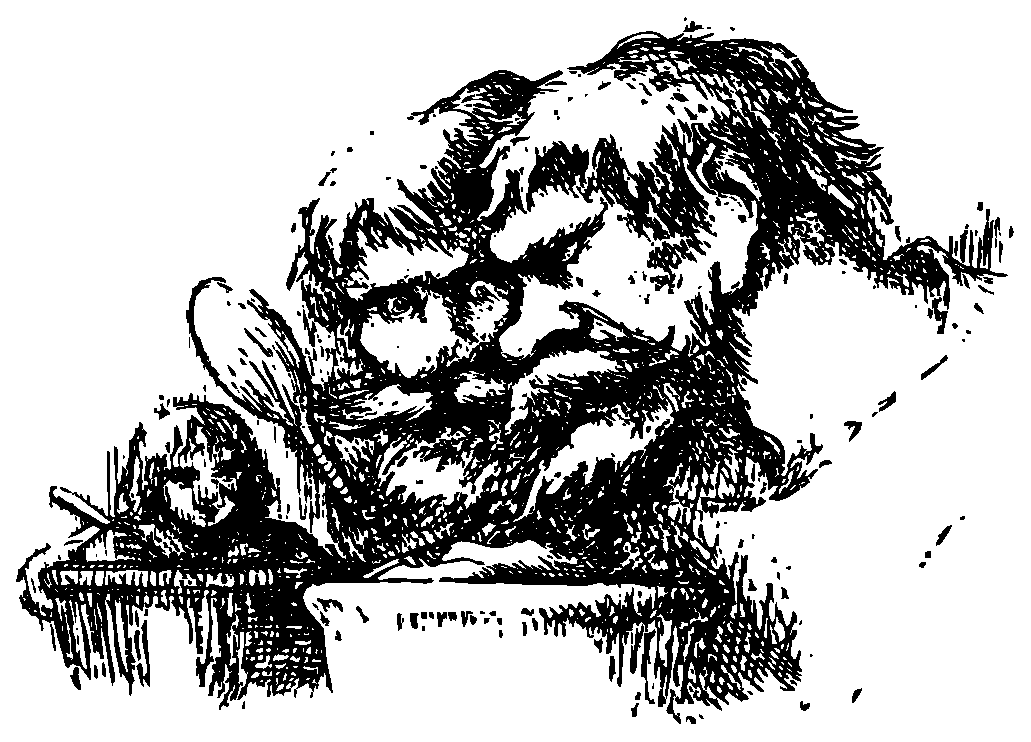
\includegraphics[scale=0.4]{../graphics/johnny_automatic_Jack_eating_with_the_giant.eps}
\end{center}

\lettrine{E}{n los capítulos anteriores} se han descrito conceptos tan importantes como: qué es \alma{}, qué son las comunidades de práctica y, sobre todo, qué tipo de \textit{software} nos puede ayudar a conseguir nuestro objetivo. En este capítulo nos centraremos en dar una visión detallada de cómo se puede implementar una comunidad de práctica con las herramientas que tiene disponible por defecto \tiki{} (sin utilizar, todavía, ningún tipo de automatización con \profiles{}). Esto nos ayudará a, por una parte, tener una visión genérica de las capacidades que nos brinda el \textit{software} (y hasta que punto podemos \q{adaptarlo} a nuestras necesidades) y por otra, a darnos cuenta de que crear comunidades de práctica es una tarea repetitiva y tediosa para un administrador.

\section{¿De qué manera podemos implementar una comunidad de práctica con \tiki{}?}

Si recordamos, en la \figureref{comunidades_de_practica} del \chapterref{estado-cuestion} aparecían múltiples comunidades de práctica (en recuadros de color verde y lila, las asignaturas de \q{Derecho Romano} y \q{Circuitos Eléctricos}, respectivamente) dentro de una plataforma wiki que era dirigida por un administrador (el recuadro azul). A continuación, en la \figureref{comunidad_de_practica_derecho_romano}, se ha cogido del ejemplo anterior la comunidad de práctica de \q{Derecho Romano} y será sobre ella donde se ilustrarán los conceptos más importantes que debemos de conocer de \tiki{} para implementar las comunidades de práctica. Hay que añadir que toda información que se presente aquí no pretende ser exhaustiva en cuanto a demostraciones de como administrar la plataforma, ya que, no es el objetivo principal de este \pfc{} hacerlo. Si bien cuando se considere oportuno, se instará al lector a buscar más información dentro de los enlaces presentados en el capítulo anterior y de los que se presenten en éste. ¡Comenzamos!

\begin{figure}
\centering
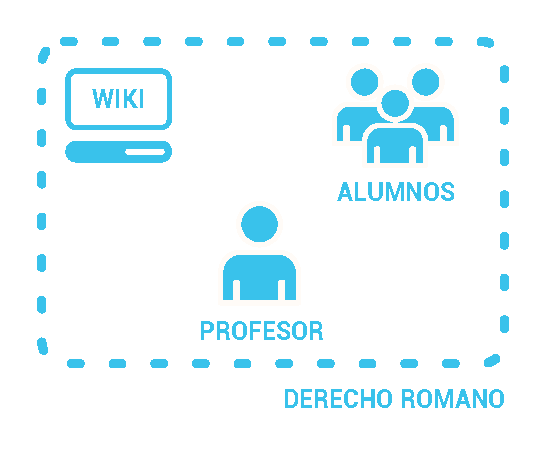
\includegraphics[width=.8\linewidth]{../graphics/fig_comunidad_de_practica_derecho_romano.eps}
\caption{La comunidad de práctica de la asignatura de Derecho Romano.}\label{fig:comunidad_de_practica_derecho_romano}
\end{figure}

\subsection{Concepto de recursos}
\label{section:concepto-recursos}

Un \textit{recurso} no es, ni más ni menos, que cualquiera de las herramientas que nos pone \tiki{} a nuestra disposición (\textit{wikis}, foros de discusión, galerías de imágenes\ldots{}) y que puede ser utilizado por las comunidades de práctica para implementar sus actividades (\figureref{comunidad_de_practica_derecho_romano_recursos}).
La creación de recursos en \tiki{} es bastante sencillo, ya que, basta con que un administrador acuda a la página de administración de la plataforma (por defecto: \url{http://localhost/tiki-admin.php?page=features}\footnote{Asumimos que tenemos \tiki{} correctamente instalado, funcionando con una base de datos habilitada para tal efecto y en nuestro caso se está ejecutando en un ordenador local, de ahí que se use \texttt{http://localhost} como dominio principal de la dirección de ejemplo \cite{web:instalacion-tiki}.}) y habilite las características que desea. (En la \figureref{panel_habilitar_recursos_tiki} vemos como se pueden activar y desactivar los diferentes recursos que posee la plataforma.) 
 Una vez que el administrador ha habilitado los recursos que desea, puede visitar la página: \url{http://localhost/tiki-admin.php} y configurar las opciones pertinentes a dicho recurso (\figureref{panel_de_recursos}).


Cabe añadir que dichos recursos son globales, es decir, sin haber cambiado ninguna opción más de la plataforma, se crearía una sola \textit{wiki} o una sola galería de imágenes o un foro. Estos elementos serían comunes a todos los usuarios (no habría todavía ningún concepto de comunidades de práctica). 

\begin{figure}
\centering
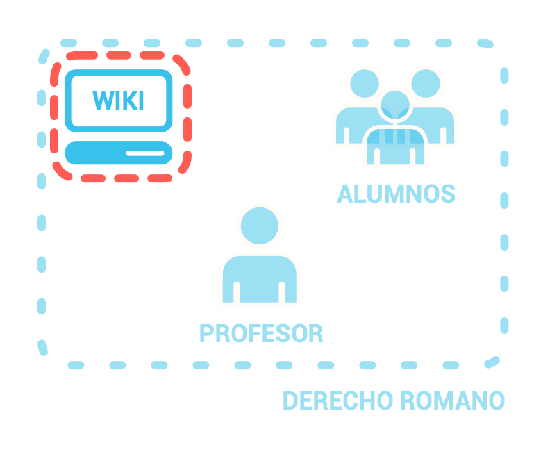
\includegraphics[width=.8\linewidth]{../graphics/fig_comunidad_de_practica_derecho_romano_recursos.eps}
\caption{Los recursos son aquellas herramientas que \tiki{} nos pone a nuestra disposición: \textit{Wikis}, Foros, Galerías de Imágenes ...}\label{fig:comunidad_de_practica_derecho_romano_recursos}
\end{figure}

\begin{figure}
\centering
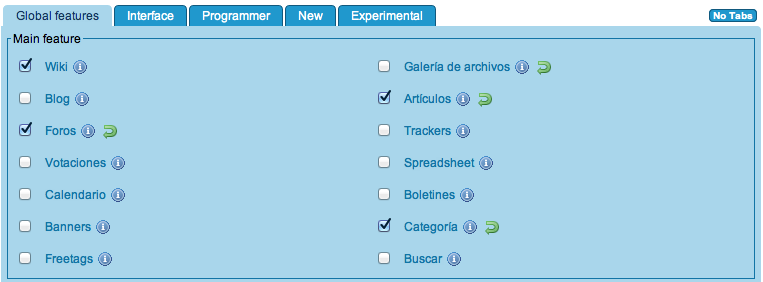
\includegraphics[width=\linewidth]{../graphics/fig_panel_habilitar_recursos_tiki.png}
\caption{Panel de habilitación de recursos en \tiki{}.}\label{fig:panel_habilitar_recursos_tiki}
\end{figure}

\begin{figure}
\centering
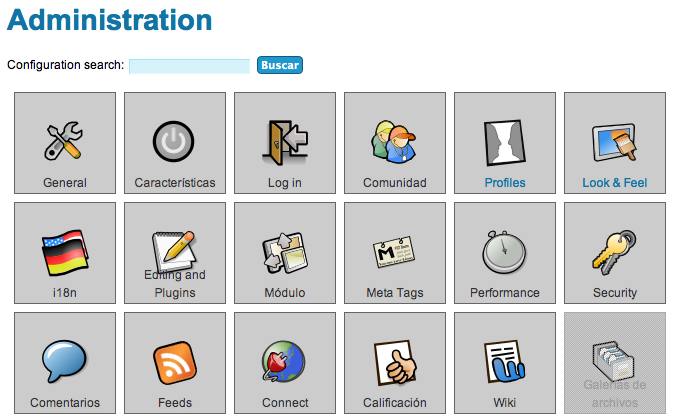
\includegraphics[width=\linewidth]{../graphics/fig_panel_de_recursos.png}
\caption{Panel de administración principal. Nos indica con transparencias si un recurso está habilitado o no (en este caso en concreto el recurso \q{galería de archivos} está desactivado). Si pinchamos en el icono del recurso nos lleva a su página de configuración.}\label{fig:panel_de_recursos}
\end{figure}

\subsection{Concepto de grupos}

\begin{figure}
\centering
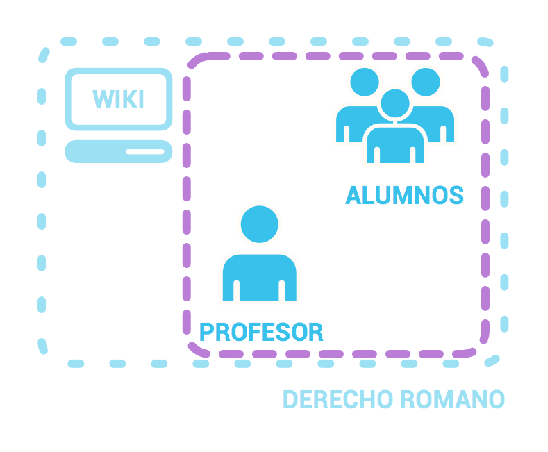
\includegraphics[width=.8\linewidth]{../graphics/fig_comunidad_de_practica_derecho_romano_grupos.eps}
\caption{Los grupos nos permiten aunar usuarios según preferencias. Pueden ser tan granulares como deseemos y un usuario puede pertenecer a uno o varios grupos.}\label{fig:comunidad_de_practica_derecho_romano_grupos}
\end{figure}

Los \textit{grupos} (como su propio nombre indica) se utilizan en \tiki{} como un contenedor donde se pueden agrupar, utilizando algún criterio de clasificación, a distintos usuarios de la plataforma. Se utilizan para múltiples propósitos pero, entre ellos, el más importante es que se les puede otorgar (o eliminar) permisos de acceso a los diferentes recursos (por ejemplo: que un determinado grupo pueda editar una página \textit{wiki} pero que a su vez no pueda subir imágenes a ésta). Esta característica nos es útil, en nuestro caso, porque podemos crear múltiples grupos que engloben a los diferentes roles que existen (profesores y alumnos) y asignarles a éstos diferentes permisos de acceso a los recursos (\figureref{comunidad_de_practica_derecho_romano_grupos} y \figureref{panel_administracion_grupos}).

\begin{figure}
\centering
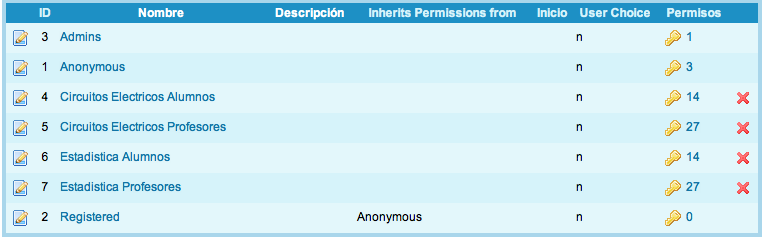
\includegraphics[width=\linewidth]{../graphics/fig_panel_administracion_grupos.png}
\caption{Panel de administración de grupos.}\label{fig:panel_administracion_grupos}
\end{figure}

Por defecto, \tiki{} genera tres grupos importantes que son tratados de manera especial por el \textit{software}: \texttt{Anonymous}, \texttt{Registered} y \texttt{Admins}. Éstos engloban a cualquier usuario de la plataforma: al primero, pertenecen todos aquellos usuarios que están visitando \tiki{} pero que no se han registrado o que no han iniciado una sesión en la plataforma; al segundo, si hacemos una traducción directa del inglés, pertenecen todos aquellos que si han iniciado una sesión en el \textit{software}; al tercero, pertenecen todos aquellos usuarios que tienen roles de administradores, es decir, los que poseen el máximo poder administrativo de la propia plataforma.  

También hay que destacar que otra de las características que poseen los grupos en \tiki{} es que se pueden crear unos dentro de otros (y montar así una jerarquía de grupos). Esto permite el que se pueda concebir un grupo cualquiera con unos permisos genéricos y luego que otros grupos hereden dichos permisos e ir restringiéndolos según se necesite. Se evita duplicar esfuerzos aunque, en nuestro caso, no utilizamos esta característica para implementar las comunidades de práctica. 

Para más información relativa a los grupos podemos visitar: \url{http://doc.tiki.org/Groups}.

\subsection{Concepto de categorías}

Al igual que con los grupos podíamos asociar a usuarios en distintos conjuntos, las \textit{categorías} es un concepto similar que funcionan de la misma manera, sólo que en lugar de agrupar usuarios permiten clasificar los recursos de \tiki{}. Cualquier recurso que existe en la plataforma es susceptible de ser categorizado incluyendo: \textit{blogs}, galerías de imágenes, artículos, encuestas, foros, páginas \textit{wiki}, galerías de archivos, etcétera. Y al igual que con los grupos, un recurso puede pertenecer a una o varias categorías y que cada categoría tenga sus propios permisos individuales (\figureref{comunidad_de_practica_categorias}).

\begin{figure}
\centering
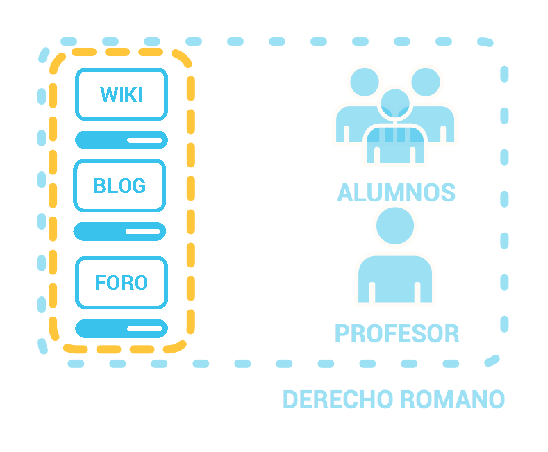
\includegraphics[width=.8\linewidth]{../graphics/fig_comunidad_de_practica_derecho_categorias.eps}
\caption{Conjunto de recursos agrupados en una categoría y que pertenecen a la comunidad de práctica de Derecho Romano.}\label{fig:comunidad_de_practica_categorias}
\end{figure}

El principal uso que se le da a las categorías es para controlar el acceso a un conjunto específico de recursos. Al establecer permisos concretos en una categoría, lo que hace es que todos los permisos globales que tenían los recursos por si solos desaparecen y son sobreescritos por los que hay en la categoría (en la siguiente sección se verá de manera más detallada como se aplican los permisos).

Las categorías también se pueden utilizar para ayudar en la navegación del sitio o para crear un conjunto de recursos relacionados por algún criterio. Por ejemplo: en la \figureref{listado_categorias} observamos que hay una categoría llamada \q{Circuitos Eléctricos}, dentro de ella estarían los recursos que pertenecen a dicha comunidad de práctica.

\begin{figure}
\centering
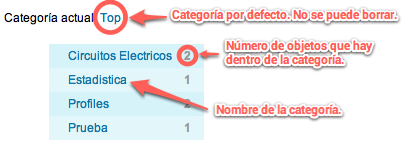
\includegraphics[scale=.8]{../graphics/fig_listado_categorias.png}
\caption{Listado de todas las categorías que se han creado en \tiki{}.}\label{fig:listado_categorias}
\end{figure}

Como sucedía con los grupos, \tiki{} crea una categoría especial denominada \texttt{Top} que es la categoría madre donde todas las demás dependerán de ella, es decir, heredarán de esa categoría. También es posible crear categorías dentro de categorías y obtener así un árbol jerárquico (aunque nosotros no exploraremos esa opción ya que no nos es necesario para poder crear las comunidades de práctica).

Las categorías en \tiki{} no vienen habilitadas por defecto, así que es tarea del administrador decidir si desea tenerlas activas o no.
Para administrarlas se debe de ir a la siguiente dirección: \url{http://localhost/tiki-browse_categories.php} y ahí nos encontraremos con el panel de la \figureref{listado_categorias}. Si se pincha en una categoría se podrá obtener información más detallada sobre ésta, los recursos que tiene asociados y los permisos que posee\ldots{} (\figureref{vista_categoria_circuitos}) 

Para averiguar más sobre las categorías podemos visitar: \url{http://doc.tiki.org/Category}.

\begin{figure}
\centering
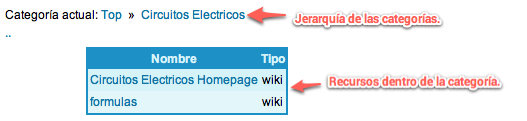
\includegraphics[scale=.8]{../graphics/fig_vista_categoria_circuitos.png}
\caption{Vista detallada de la categoría Circuitos Eléctrico y sus recursos asociados.}\label{fig:vista_categoria_circuitos}
\end{figure}

\subsection{Concepto de permisos}
\label{section:concepto-permisos}

\begin{figure}
\centering
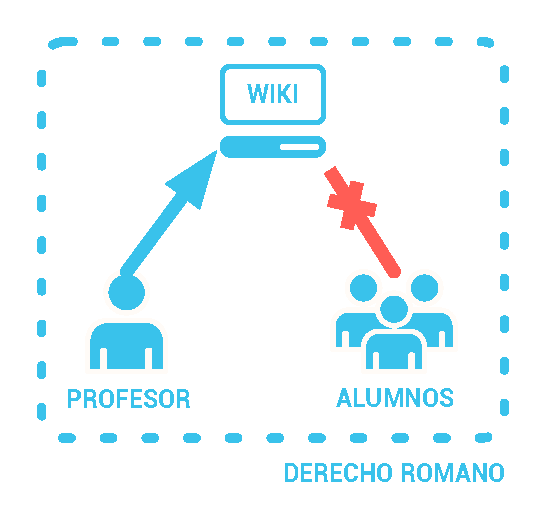
\includegraphics[width=.8\linewidth]{../graphics/fig_comunidad_de_practica_derecho_permisos.eps}
\caption{Concepto de lo que son los permisos en \tiki{}.}\label{fig:concepto_permisos}
\end{figure}

Los \textit{permisos} son una de las herramientas más poderosas que posee \tiki{} y es con ellos con los que podemos crear, junto con las perspectivas \sectionref{concepto_perspectivas}, el concepto de las comunidades de práctica. Un administrador de la plataforma puede decidir quién y bajo qué circunstancias un usuario o un grupo puede acceder a un recurso y modificarlo. El esquema de permisos de \tiki{}, sobre todo al principio, puede parecer un poco caótico (en parte debido a como se ha implementado el panel de administración), pero, una vez acostumbrados podemos personalizar la plataforma a nuestro gusto de maneras que no habíamos imaginado. Se intentará dar la mejor explicación posible aunque, no obstante, la mejor forma de aprender sobre esta herramienta es realizando pruebas sobre una instalación de \tiki{} destinada para tal efecto.

Para entender como funcionan los permisos antes hay que asumir una serie de ideas (muchas de ellas ya han sido expuestas en las anteriores secciones, pero, se volverán a repetir con el fin de clarificar al máximo los conceptos):

\begin{itemize}
\item Referente a los recursos, es decir, las \textit{wikis}, los \textit{blogs}, los foros\ldots{} pueden tener permisos de manera individual a los que tengan los grupos y las categorías.   
\item Referente a las categorías:
      \begin{itemize}
      \item Los recursos pueden ser categorizados.
      \item Una categoría se puede asignar a un grupo específico.
      \item Los permisos que se le otorguen a una categoría garantiza a los miembros del grupo el derecho a poder ver y a editar el contenido de dicha categoría.
      \item Una categoría puede pertenecer a otra categoría.
      \item Si a una categoría no se le especifican permisos concretos, se aplican los genéricos.
      \end{itemize}
  \item Referente a los grupos:
      \begin{itemize}
       \item Cada grupo puede tener un acceso personalizado a todas las características de \tiki{}.
       \item Los usuarios pueden estar en uno o en múltiples grupos.
       \item Los grupos pueden tener \q{grupos dentro de otros grupos}.
       \item Los permisos se añaden a los grupos en general, \textsc{no} a los usuarios.
        \item Si a un grupo no se le especifican permisos concretos, se aplican los genéricos.
        \item Por defecto, \tiki{} genera tres grupos de manera predeterminada:
          \begin{itemize}
            \item \texttt{Anonymous}: Los usuarios que no tienen una cuenta en la plataforma o que no han iniciado una sesión con su usuario pertenece a este grupo.
            \item \texttt{Registered}: Cualquier usuario que ha iniciado una sesión en el sistema, independientemente de que pertenezca a otro grupo, por defecto pertenecen a este grupo.
            \item \texttt{Admins}: Grupo encargado de la administración, como ya comentamos anteriormente. 
          \end{itemize}
      \end{itemize}
\end{itemize}

\parabreak

En la documentación oficial podemos encontrar un listado de todos los permisos que posee \tiki{} \cite{web:listado-permisos} (conviene visitar ese enlace para tener una idea aproximada de la cantidad de permisos que existen). El formato que utilizan para definir un permiso es de la siguiente manera: \texttt{tiki\_p\_} + \texttt{nombre\_del\_permiso}. Ponemos tres ejemplos:

\begin{itemize}
\item \textit{tiki\_p\_edit}: Permiso que permite editar una página \textit{wiki}.
\item \textit{tiki\_p\_admin}: Permiso que garantiza a un usuario derechos de administración.
\item \textit{tiki\_p\_upload\_picture}: Permiso que permite subir una imagen a una página \textit{wiki}.
\end{itemize}

Si queremos tener éxito a la hora de manejar los permisos, es importante conocer el orden en el que se deben aplicar ya que, si no, no obtendremos los resultados deseados (y sucede con bastante frecuencia). A continuación, se muestran éstos ordenados de mayor a menor importancia (\figureref{esquema_permisos_circular}): 

\begin{figure}
\centering
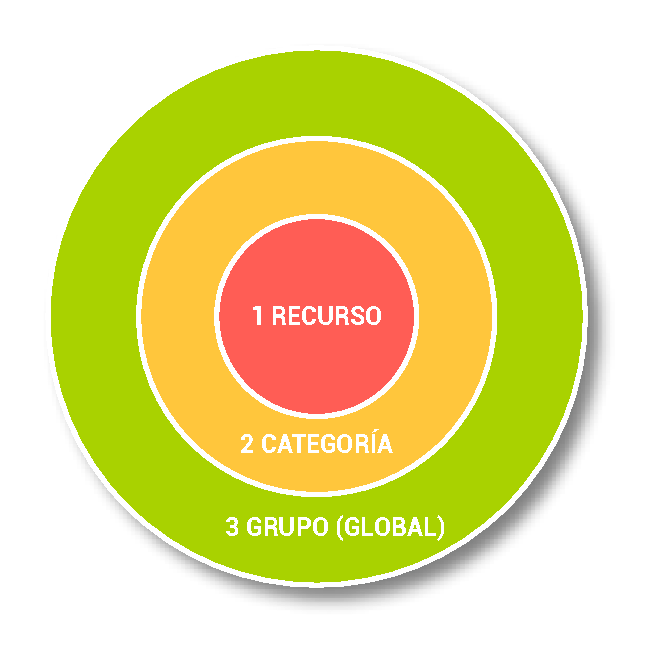
\includegraphics[width=.8\linewidth]{../graphics/fig_esquema_permisos_circular.eps}
\caption{Orden en el que se aplican los permisos en \tiki{}. Imagen inspirada en la documentación oficial \url{http://twbasics.keycontent.org/img/wiki_up/tiki_permissions.png}.}\label{fig:esquema_permisos_circular}
\end{figure}

\begin{itemize}
\item \textit{Recurso}: Los permisos de un recurso definen que acciones puede realizar un usuario para un recurso en concreto. Por ejemplo, podríamos tener una página \textit{wiki} que \textsc{no} permitiese subir ficheros, o que \textsc{no} permitiese la edición de su contenido, y dichos permisos serían los que imperasen, independientemente de que dicha \textit{wiki} estuviese categorizada en una categoría que permite editar contenidos \textit{wiki} o subir ficheros o de que el grupo, en general, pueda hacerlo.

 \item \textit{Categoría}: Los siguientes permisos en tenerse en cuenta son los relativos a que el recurso pertenezca a una categoría. Si, por ejemplo, en la categoría se describe que \textsc{no} se pueden subir imágenes a las páginas \textit{wikis} de esa categoría, y en cualquier página \textit{wiki} no existe un permiso que contradiga dicha regla, entonces se podrán subir imágenes. Recordamos que no puede existir un recurso que no esté asignado a ninguna categoría ya que, por defecto, pertenece a la categoría \texttt{Top} y dicha categoría también tiene unos permisos por omisión (que podemos modificar si así deseamos).

 \item \textit{Grupo (y los permisos globales)}: Los permisos de grupo son los últimos en aplicarse y son los que menos preferencia tienen en caso de que existan permisos contradictorios en los de categoría y los de recurso. Por otra parte, como cualquier usuario pertenece a un grupo, bien sea \texttt{Registered} o \texttt{Anonymous} sin contar con que esté en otros grupos se garantiza que, como mínimo, haya unos permisos globales básicos.  
\end{itemize}

A modo de resumen de lo expuesto anteriormente podemos decir que, si no hay una contradicción en los permisos, estos se heredan de arriba a abajo, es decir, Grupo \char"25B7~ Categoría \char"25B7~ Recurso. En cambio, si hay algún permiso que contradiga alguno de los anteriores, éstos sobreescriben de abajo a arriba, es decir, Grupo \char"25C1~ Categoría \char"25C1~ Recurso.

Si queremos obtener más información para administrar los permisos de las categorías, debemos acudir a la siguiente dirección: \url{http://localhost/tiki-admin_categories.php}.

\begin{figure}
\centering
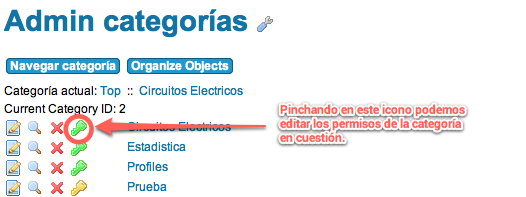
\includegraphics[width=.8\linewidth]{../graphics/fig_asignacion_permisos_llave_verde.png}
\caption{Listado de todas las categorías disponibles. Para editar los permisos de una categoría hay que pinchar en el icono de la llave verde.}\label{fig:asignacion_permisos_llave_verde}
\end{figure}

\begin{figure}
\centering
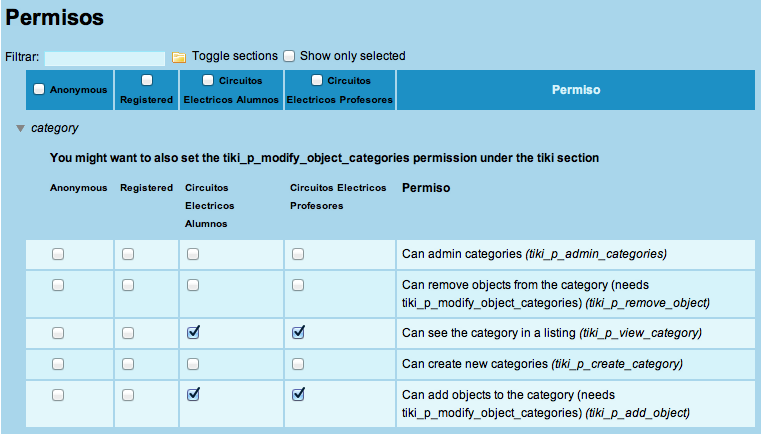
\includegraphics[width=\linewidth]{../graphics/fig_asignacion_permisos_categoria.png}
\caption{Listado de los posibles permisos que se pueden asignar a la categoría (en la imagen no se muestra toda la información). Como se puede apreciar, se pueden asignar permisos de manera independiente para cada grupo.}\label{fig:asignacion_permisos_categoria}
\end{figure}

\subsection{Concepto de preferencias}
\label{section:concepto-preferencias}

Como ya se ha comentado anteriormente, \tiki{} posee más de 1500 configuraciones y opciones posibles divididas en varios paneles de administración. Las \textit{preferencias} (como su propio nombre indica) nos permiten  configurar la plataforma a nuestro gusto. Será una tarea del administrador decidir qué \q{características} desee que estén activas, pasando por los recursos, como por la configuración de los envíos de correo a los usuarios, que apariencia externa tiene la plataforma, etcétera.

Uno de los problemas que plantea \tiki{} respecto a la administración es que tiene demasiadas posibilidades de configuración. Hay demasiados paneles, demasiadas casillas para activar y desactivar y múltiples opciones. Normalmente la tarea de configurar la plataforma se suele realizar la primera vez que se instala en el servidor. Este proceso puede incluso hasta llevar varias horas en completarse dependiendo, claro está, de las necesidades concretas de cada instalación y de la pericia que tenga manejando el \textit{software} el administrador.

Las principales desventajas que encontramos, aparte de la pérdida de tiempo que supone configurar, es que un usuario tiene que conocerse bien la plataforma (o al menos haber leído mucha información, o haber probado a base de ensayo y error). Además, las configuraciones no se pueden reutilizar, es decir, si disponemos de dos plataformas y queremos compartir la configuración que tenemos en una y llevarla a la otra de forma directa, no vamos a ser capaz de poder hacerlo.

Por fortuna los \profiles{} solventan de manera elegante todos estos inconvenientes y en el \chapterref{gestion-dinamica} veremos como se ha creado un \profile{} que configura \alma{} en muy poco tiempo. Pero para ello, antes debemos conocer un poco el funcionamiento básico de las preferencias en \tiki{}.

De forma interna las preferencias se guardan en tres tablas importantes de la base de datos que hay que conocer:

\begin{itemize}
 \item \texttt{tiki\_preferences}
 \item \texttt{tiki\_perspective\_preferences}
 \item \texttt{tiki\_user\_preferences}
\end{itemize}

\begin{figure}
\centering
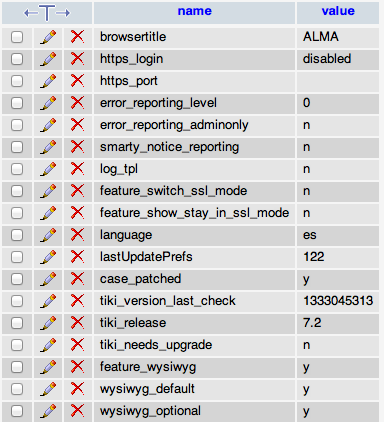
\includegraphics{../graphics/fig_valores_preferencias.png}
\caption{Algunos valores almacenados en la tabla \texttt{tiki\_preferences}.}\label{fig:valores_preferencias}
\end{figure}

La principal y la más importante es la tabla \texttt{tiki\_preferences}, ya que, es la encargada de almacenar los valores principales de todas las posibles configuraciones que pueden existir en \tiki{}. Dicha tabla almacena por ejemplo: el idioma que debe mostrar la aplicación, las \q{características} que hay habilitadas, la configuración para el envío de notificaciones de correo, el nombre de la plataforma\ldots{} Es decir, cualquier opción que modifiquemos en el panel de administración queda almacenado ahí.  
La estructura relacional de esta tabla es sencilla: almacena el nombre de la preferencia y su valor asociado.

\begin{figure}[h!]
\begin{pyglist}[language=sql]

  CREATE TABLE `tiki_preferences` (
    `name` varchar(40) NOT NULL default '',
    `value` text,
    PRIMARY KEY (`name`)
  ) ENGINE=MyISAM;
  
\end{pyglist}
\caption{Estructura de la tabla \texttt{tiki\_preferences}.}
\end{figure}
  
La librería de código que se encarga de almacenar y recoger los datos guardados en dicha tabla se llama \texttt{Prefslib.php} y dicho \textsc{php} se encuentra en la carpeta \texttt{lib/} al descargar el código fuente\footnote{Para más información sobre como está organizado el código fuente de \tiki{} recomendamos al lector la lectura del \appendixref{organizacion-codigo} al final del documento.}.

De forma genérica, y sin entrar en detalles muy concretos, cuando un usuario realiza una petición a \tiki{} esa librería extrae los datos de la tabla \texttt{tiki\_preferences} y los almacena en un \texttt{array asociativo} \cite{web:documentacion-php-arrays}. De esta manera podemos obtener los valores que deseemos utilizando una simple sentencia de programación de \php{}:

\begin{figure}[h!]
\begin{pyglist}[language=php]

  <?php
  print($prefs['tiki_release']); // Y obtendríamos el número de versión de TikiWiki.
      
\end{pyglist}
\caption{Un ejemplo de lo que contiene el array \code{\$prefs} (que son todos los datos de la tabla \texttt{tiki\_preferences}).}
\end{figure}

La tabla \texttt{tiki\_user\_preferences}, como su nombre indica, guarda, de manera análoga a como lo hace \texttt{tiki\_prerefences}, las preferencias que tienen los usuarios. Esto les permite configurar a cada uno que opciones desean de manera individual, es decir, cada usuario tiene sus propias preferencias. Por ejemplo: uno se podría llamar Pepito Pérez y su alias \texttt{pperez} y otro John Doe y su alias \texttt{jdoe} y esos datos se guardan en esa tabla.

La tabla \texttt{tiki\_perspective\_preferences} funciona de manera análoga a las anteriores, pero, su uso es diferente puesto que está ligado al concepto de las perspectivas. En la siguiente sección hablaremos más detalladamente de esta última tabla.

Tener un conocimiento de como se almacenan las preferencias y como se emplean nos ayuda posteriormente a poder desarrollar mejor los \profiles{} que configuren una instalación de \tiki{}.

Hay que decir que este tipo de información no se encuentra en ninguno de los canales oficiales presentados, por lo que recomendamos al lector interesado que explore de manera profunda lo que se ha presentado aquí si quiere obtener un conocimiento avanzado de como funciona internamente \tiki{}.

\subsection{Concepto de perspectivas}
\label{section:concepto_perspectivas}

\begin{figure}
\centering
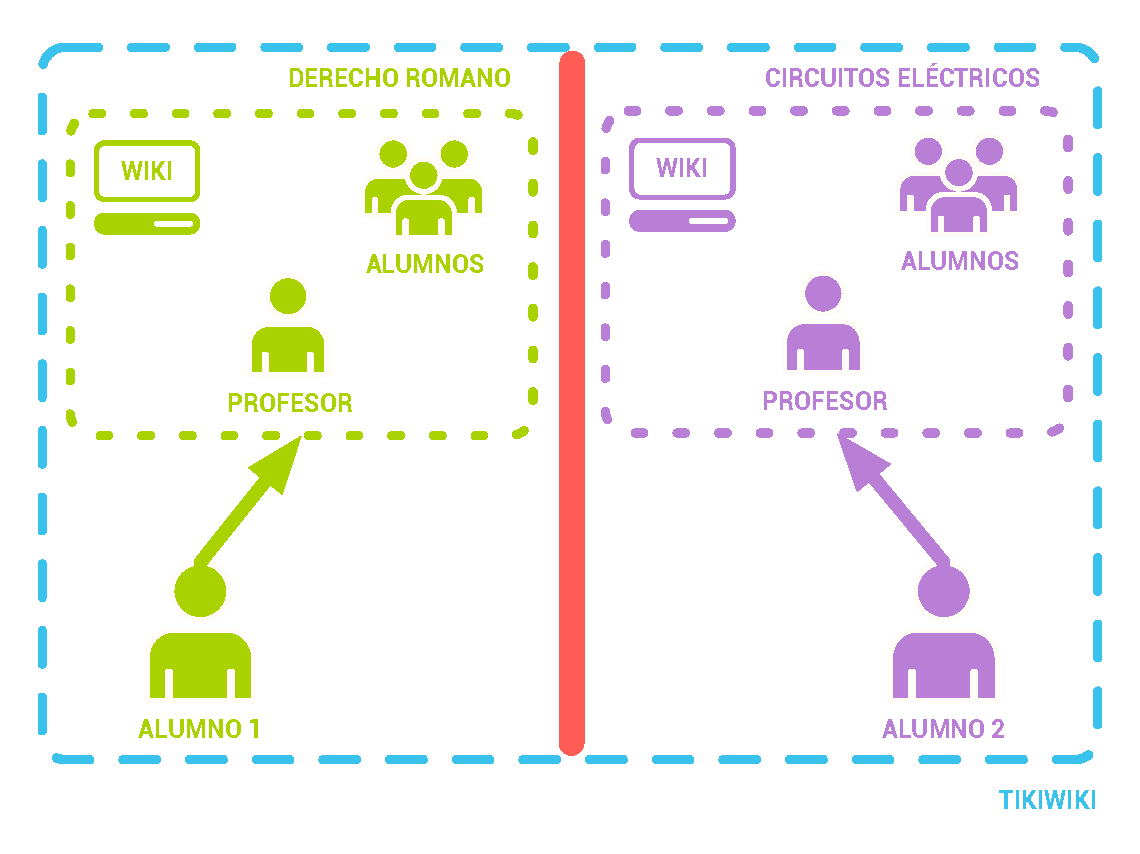
\includegraphics[width=.8\linewidth]{../graphics/fig_comunidad_de_practica_perspectivas.eps}
\caption{Ejemplo de dos posibles alumnos en el cual el Alumno 1 desconoce que existe la comunidad de práctica de Circuitos. Las perspectivas en \tiki{} nos permiten aislar de forma transparente comunidades de práctica dentro de una misma instalación.}\label{fig:comunidad_de_practica_perspectivas}
\end{figure}

Las \textit{perspectivas} son un concepto que apareció en las últimas versiones de \tiki{} (concretamente en la versión 4) y con las cuales somos capaces de implementar la separación entre diferentes comunidades de práctica utilizando la misma instalación de \textit{software}. Esto nos interesa mucho a la hora de implementar las comunidades de práctica, ya que, de esta manera podemos hacer que \tiki{} muestre solo cosas relevantes a un determinado grupo y no a otro (a un alumno concreto no le importa ver otras asignaturas que no sean a las que él está matriculado, \figureref{comunidad_de_practica_perspectivas}).

Además, aparte de separar diferentes comunidades de práctica, las perspectivas nos permiten personalizar \tiki{} y adaptarlo a las necesidades concretas de cada asignatura. Por ejemplo: en la vida real cuando un alumno entra en un aula puede encontrar un determinado color de pared, la distribución de las sillas tienen una forma determinada, la iluminación se manifiesta de una forma concreta\ldots{} y todas estas características son completamente diferentes en otro aula. Podemos replicar de manera \q{psicológica} este mismo comportamiento cambiando por ejemplo el logotipo principal de \tiki{} por el de la asignatura Circuitos cuando el alumno entra dentro de la comunidad de práctica, o cambiar el color del tema visual que se está utilizando por ejemplo de azul a verde. Lo positivo es que estos \q{efectos} duran mientras el usuario esté dentro de una comunidad de práctica, cuando la abandona, los cambios se revierten a los que había previamente (al igual que cuando un alumno abandona un aula el entorno previo permanece igual, \figureref{explicacion_perspectivas}).

\begin{figure}
\centering
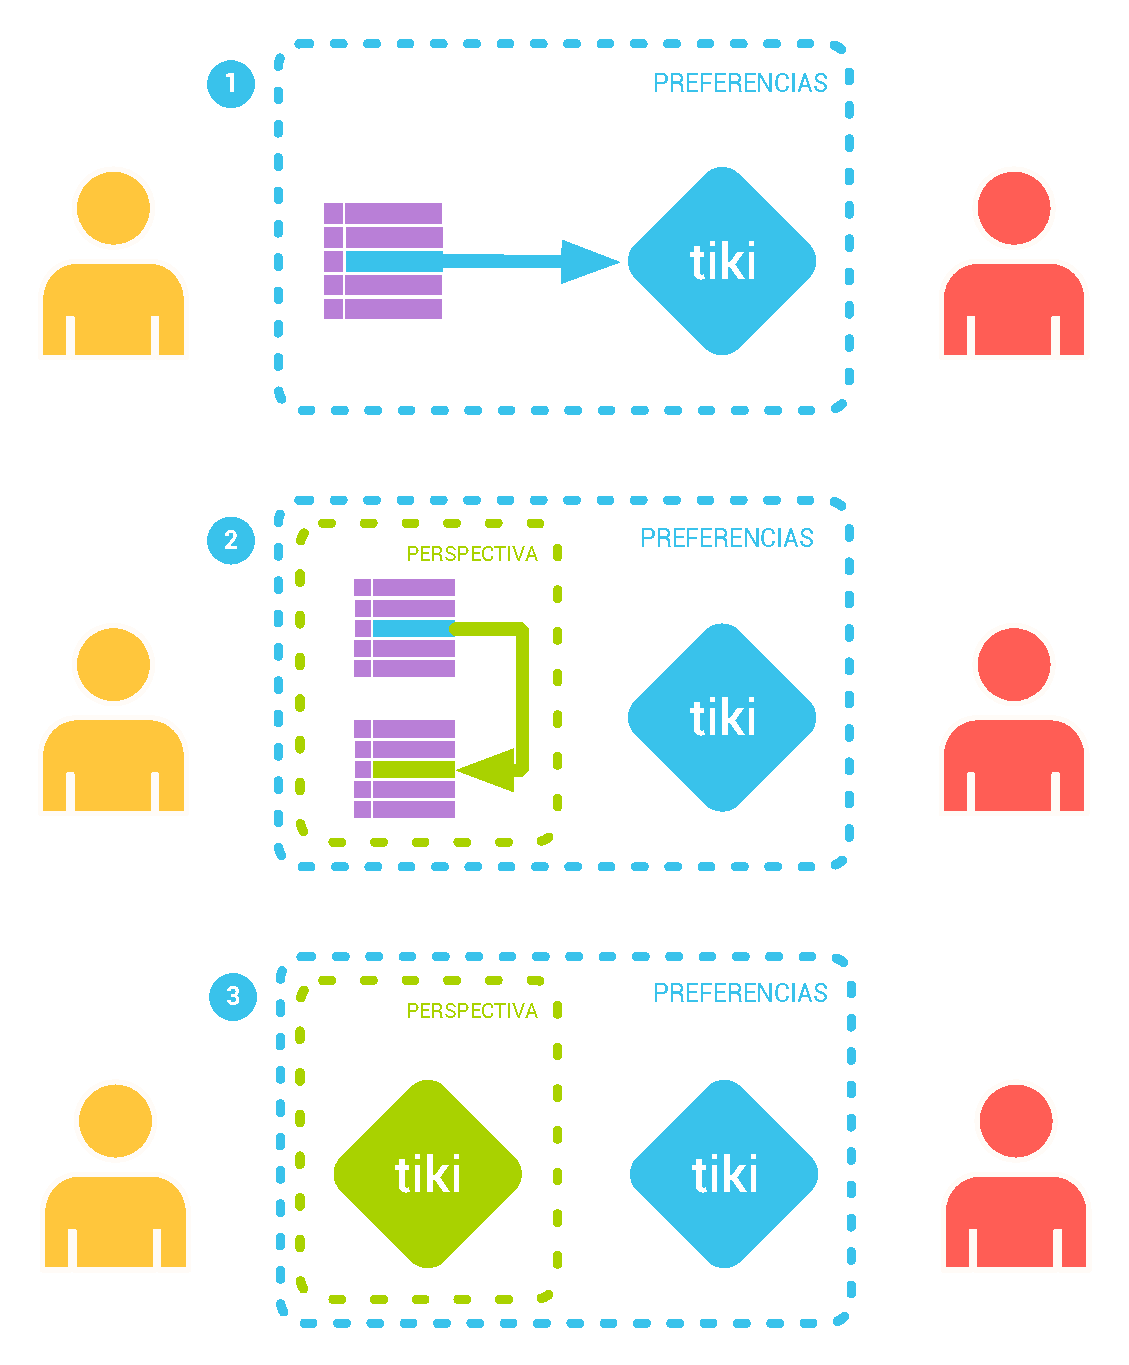
\includegraphics[width=.9\linewidth]{../graphics/fig_explicacion_perspectivas.eps}
\caption{Supongamos que existen dos usuarios y que pertenecen a dos comunidades de práctica diferentes. En el primer ejemplo (denotado en el gráfico con el número uno) los dos ven el color del logotipo de \tiki{} azul, ya que, así lo indica sus preferencias genéricas. En un instante de tiempo \texttt{t + 1} el usuario amarillo decide entrar en una comunidad de práctica. Dicha comunidad de práctica posee una perspectiva que cambia la preferencia de que el logotipo sea de color azul a que sea verde (se puede observar en el gráfico número dos como se ejecuta el cambio internamente). El usuario amarillo acaba entrando en la comunidad de práctica (gráfico número tres) y ya lo que él observa es que el logotipo ha cambiado de color, sin embargo, para el usuario de color rojo al no pertenecer a la misma comunidad de práctica (y, por consiguiente ,al no haber ejecutado la perspectiva asociada) observa que el color del logotipo sigue siendo azul. En el momento en el que el usuario amarillo abandone la comunidad de práctica, todos los cambios que ha efectuado la perspectiva se revierten y se volvería a estar en el gráfico número uno.}\label{fig:explicacion_perspectivas}
\end{figure}

El funcionamiento de las perspectivas es sencillo, simplemente sobreescriben temporalmente cualquiera de las 1500 preferencias que existen en \tiki{}. Recordamos al lector que las preferencias se guardaban en la tabla \texttt{tiki\_preferences}. Éstas en el momento en el que se activan, cargan y ejecutan las preferencias modificadas de la tabla \texttt{tiki\_perspective\_preferences}. Por lo tanto es importante saber que cualquier preferencia que exista en la tabla \texttt{tiki\_preferences} es susceptible de ser modificada por una perspectiva\footnote{Esto es importante saberlo ya que a la hora de implementar \profiles{} en la documentación oficial de \tiki{} no se listan todas las opciones posibles. La mejor solución es acudir a la tabla de las preferencias y ver que valores hay ahí.}. 

Las perspectivas pueden ser administradas desde la interfaz de \tiki{}, si el administrador visita el siguiente enlace: \url{http://localhost/tiki-edit_perspective.php} se encontrará con lo que muestra la \figureref{panel_administracion_perspectivas}; si decide editar las preferencias que modificará una perspectiva entonces verá lo que muestra la \figureref{detalle_modificacion_preferencias}.

\begin{figure}
\centering
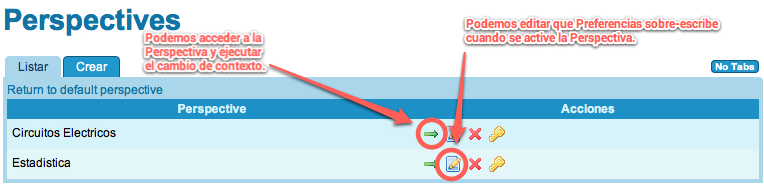
\includegraphics[width=\linewidth]{../graphics/fig_panel_administracion_perspectivas.png}
\caption{\tiki{} permite crear, editar y borrar perspectivas. Hay que reconocer que la interfaz web no es la forma más cómoda de administrar las perspectivas, aunque para ediciones sencillas sirve perfectamente.}\label{fig:panel_administracion_perspectivas}
\end{figure}

\begin{figure}
\centering
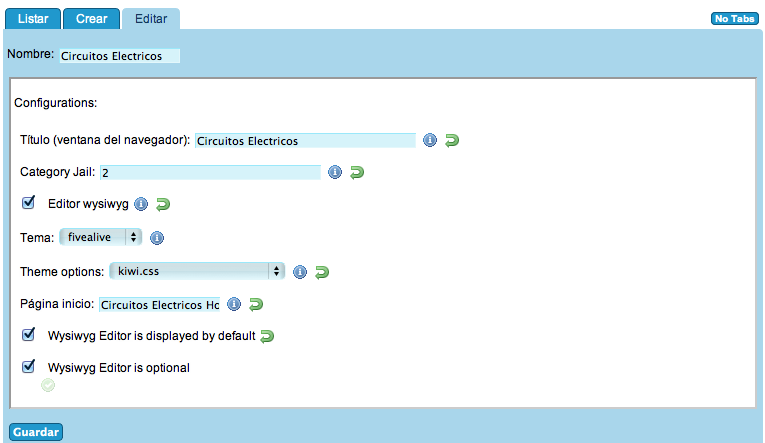
\includegraphics[width=\linewidth]{../graphics/fig_detalle_modificacion_preferencias.png}
\caption{Aquí se listan las preferencias que se activarán en la comunidad de práctica de la asignatura de Circuitos Eléctricos. Han sido generadas de forma automática con un \profile{} (añadir preferencias de forma manual es un proceso tedioso).}\label{fig:detalle_modificacion_preferencias}
\end{figure}

Para encontrar más información relativa a las perspectivas nada mejor que acudir a la documentación oficial \url{http://doc.tiki.org/Perspectives}.

\subsection{Concepto de menús}

\begin{figure}
\centering
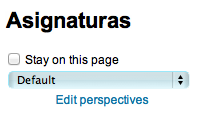
\includegraphics{../graphics/fig_menu_perspectivas.png}
\caption{Ejemplo de menú que se puede utilizar para cambiar las perspectivas y cambiar de comunidad de práctica de manera dinámica.}\label{fig:menu_perspectivas}
\end{figure}

\tiki{} tiene un gestor de creación de menús de manera que podemos generar menús que en nuestro caso nos permiten cambiar de manera dinámica las perspectivas y listar a las comunidades de práctica a las que pertenece el usuario. Esto nos permite que el usuario cambie de comunidad de práctica de manera rápida y sencilla, y al activarse la perspectiva asociada a dicha comunidad, cambiará la experiencia en \tiki{} de manera acorde. Es como si un alumno cambiase de aula (\figureref{menu_perspectivas}).

Por otra parte los menús tienen mucho más usos que para listar simplemente perspectivas. Si queremos administrar y crear menús, debemos ir a la siguiente dirección: \url{http://localhost/tiki-admin_menus.php} (\figureref{admin_menus}).

\begin{figure}
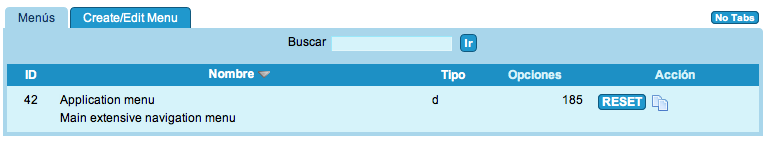
\includegraphics[width=\linewidth]{../graphics/fig_admin_menus.png}
\caption{Panel de administración de menús. Se pueden crear, editar y borrar. Hay una cantidad inmensa de opciones, más información en \url{http://doc.tiki.org/Menu+HOWTO}.}\label{fig:admin_menus}
\end{figure}

\section{¿Qué hemos aprendido de todo lo comentado en el capítulo?}

A lo largo de este capítulo hemos hecho un recorrido a las características más importantes que tiene \tiki{} que nos sirven para implementar una comunidad de práctica\footnote{De hecho en la documentación oficial de \tiki{} encontramos el concepto de \texttt{Workspaces} (\url{http://doc.tiki.org/Workspace}) que es básicamente lo que nosotros hemos denominado como comunidades de práctica. Y uno de los ejemplos es la creación manual de un \texttt{Workspace} similar a lo que hemos realizado aquí.}. Si bien, en cada sección no se ha profundizado con mucho detalle, en parte, porque si no se podrían rellenar muchas hojas presentando conceptos que el lector será capaz de descubrir fácilmente en el momento que decida utilizar la plataforma. Aún así, podemos extraer una idea importante: crear comunidades de práctica conlleva mucho tiempo y es una tarea en la que se pueden cometer errores fácilmente, puesto que, la complejidad crece de manera lineal conforme haya más comunidades de práctica a crear. Y eso, sin mencionar de tener que administrar dichas comunidades. Por lo tanto, los \profiles{} se postulan como una herramienta útil que nos ahorra tener que crear todas estas opciones de manera manual. En la siguiente parte descubriremos todo lo necesario para poder conseguir nuestro objetivo principal: liberar al administrador de las tareas repetitivas y aburridas.
